%------------------------------------------------
% Quick reference. 
%------------------------------------------------
%
% Для вставки картинок:
%
%--------         Комманда
%
%\begin{figure}[H]
%	\includegraphics{img_name}
%	\caption{some caption}
%	\label{some_pic}
%\end{figure}
%
%--------        Переменные
%
% img_name     <- Название картинки в папке img.
% some_caption <- подпись картинки.
% label        <- лейбл нужен для ссылок на картинку.
% H            <- расположение картинки на странице.
%
%--------         Пример
%
%\begin{figure}[H]
%	\includegraphics{pic1.jpg}
%	\caption{График зависимости чего-то там}
%	\label{grapics1}
%\end{figure}
%
%------------------------------------------------
%
% Для референса по лейблу:
%
%--------         Комманда
%
% Для ссылки используется \eqref{ref}.
%
%--------        Переменные
%
% ref          <- указанный лейбл в директиве \label{ref}
%                 Ссылку можно сделать на любой объект имеющий \label{•}
%
%--------         Пример
%
% \eqref{graphics1}
%
% Ссылка на источники [\ref{src_spectral_wiki}]
%
%------------------------------------------------
%
% Для листинга кода:
%
%--------         Комманда
%
% \lstinputlisting[language=lang,mathescape=true]{src}
%--------        Переменные
%
% lang         <- язык на котором написан исходный код, например "python" или "C++".
% mathescape   <- если в исходниках есть формулы LaTeX, то они будут представлены как формулы.
% src          <- путь до файла исходников.
%
%--------         Пример
%
% \lstinputlisting[language=C++,mathescape=false]{./src/bullshit.cpp}
%
%------------------------------------------------
%
% Для вставки таблиц:
%
%--------
%\begin{table}[H]
%	\centering
%	\caption{ capt }
%	\begin{tabularx}{0.9\textwidth}{ | Y | Y | }
%		\hline
%		lines
%	\end{tabularx}
%	\label{tab1}
%\end{table}
%--------
% caption      <- Подпись таблицы.
% tab1         <- лейбл нужный для ссылки на таблицу.
% | Y | Y |    <- количество и формат столбцов.
% Y            <- Тип столбца.
%                 В данном случае определены кастомные столбцы Y (Спасибо Максиму Наумову)
% |            <- обозначает границы столбца.
%                 То есть, если будет указано |Y Y|, то столбцы внутри строк разделены не будут.
% H            <- То же самое, что и у картинок.
% lines        <- непосредственно элементы таблицы.
%                 Разделяются знаком "&", оканчивать каждую строку лучше \\ \hline
%
%--------         Пример
%\begin{table}[H]
%	\centering
%	\caption{ capt }
%	\begin{tabularx}{0.9\textwidth}{ | Y | Y | }
%		\hline
%		str1 & str2 \\ \hline
%		str1 & str2 \\ \hline
%		str1 & str2 \\ \hline
%		str1 & str2 \\ \hline
%		str1 & str2 \\ \hline
%	\end{tabularx}
%	\label{tab1}
%\end{table}
%------------------------------------------------

\documentclass[14pt, a4paper, fleqn]{extarticle}

\makeatletter
\renewcommand*\l@section{\@dottedtocline{1}{1.5em}{2.3em}}



%\includegraphics{universe}

\usepackage[utf8]{inputenc}
\usepackage[T2A]{fontenc}
\usepackage[russian]{babel} % указывает язык документа
\usepackage[left=3cm,right=2cm,top=2cm,bottom=2cm,bindingoffset=0cm]{geometry}
\usepackage{lastpage}
\usepackage{fancyhdr}
\usepackage{titlesec}
\usepackage{multirow}
\usepackage{graphicx} % для вставки картинок
\usepackage[intlimits]{mathtools} % математические дополнения
\usepackage{amssymb}
\usepackage[tableposition=top]{caption}
\usepackage{subcaption}
\usepackage{indentfirst}
\usepackage{pythonhighlight}
\usepackage{listings}
\usepackage{tabularx}
\usepackage{tabulary}
\usepackage{multirow}
\usepackage{xcolor,colortbl}
\usepackage{float}
\usepackage[figure,table]{totalcount}
\usepackage{diagbox}
\usepackage[german=guillemets]{csquotes}
\usepackage{fontspec} 
\usepackage{enumitem}
%\usepackage{mathptmx}% http://ctan.org/pkg/mathptmx
%\usepackage{showframe}
\usepackage{hyperref}

\setlength{\parindent}{1.2cm}

\setlength{\mathindent}{1.2cm}

\defaultfontfeatures{Ligatures={TeX},Renderer=Basic} 
\setmainfont[Ligatures={TeX,Historic}]{Times New Roman}

%\setlist[enumerate]{itemindent=\dimexpr\labelwidth+\labelsep\relax,leftmargin=0pt}

%\setlength{\section*}{0.5cm}
%\usepackage{minted}
%\usepackage{fancyvrb}
%\usepackage{newtxtext}

%\titleformat{\section}[hang]{\bfseries\LARGE\centering}{}{1em}{}

%\setlist[enumerate]{itemindent=\dimexpr\labelwidth+\labelsep\relax,leftmargin=0pt}
\setlist[enumerate,itemize]{leftmargin=0pt,itemindent=1.7cm}
\titlespacing*{\section}{0.6cm}{1ex}{1em}
\titleformat{\section}{\bfseries\centering}{\thesection}{0.5em}{\MakeUppercase}
\titleformat{\subsection}[block]{\bfseries\hspace{1em}}{\thesubsection}{0.5em}{}
%\setlength{\subsection*}{1.5cm}
%\setlength{\parindent}{4em}

%\setlength{\parindent}{1.5cm}

\captionsetup[figure]{name={Рисунок},labelsep=endash, skip=5pt}
\captionsetup[table]{name={Таблица},labelsep=endash,singlelinecheck=false, skip=5pt}


%\renewcommand{\baselinestretch}{1.5}
\linespread{1.5} % полуторный интервал
\frenchspacing
\graphicspath{ {images/} }

%-------------------------------------------
% Ссылки в оглавлении
%-------------------------------------------

\hypersetup{
    colorlinks,
    citecolor=black,
    filecolor=black,
    linkcolor=black,
    urlcolor=black
}

%-------------------------------------------
% Стиль футеров и хедеров
%-------------------------------------------

\pagestyle{fancy}
\fancyhead[L, R]{}
\fancyfoot[L]{}
\fancyfoot[R]{}
\renewcommand{\footrulewidth}{0pt}
\renewcommand{\headrulewidth}{0pt}

%\renewcommand\subsectionfont{\normalfont\normalsize\bfseries}

\def\l@subsection{\@dottedtocline{2}{3.8em}{3.2em}}
\setcounter{tocdepth}{2}
% Для листинга

\lstset{
basicstyle=\footnotesize\ttfamily,
columns=fullflexible,
keywordstyle=\color{blue},
%frame=single,
breaklines=true,
numberstyle=\tiny\color{mygray},
postbreak=\mbox{\textcolor{red}{$\hookrightarrow$}\space},
showstringspaces=false,
}

\newcolumntype{Y}{>{\centering\arraybackslash}X}

%\renewcommand{\theenumi}{\the}
\newcommand{\incpic}[3]{
	\begin{figure}[H] 
		\begin{center} 
			\includegraphics[height=0.6\textwidth]{#1} 
			\caption{#2}
			\label{#3} 
		\end{center}
	\end{figure} 
}

\begin{document}

\pagenumbering{arabic}

\setcounter{page}{3}
%\setcounter{tocdepth}{3}
\setcounter{secnumdepth}{3}

%------------------------------------------------
% Реферат
%------------------------------------------------
\phantomsection
\section*{РЕФЕРАТ}
{
	{\bf Выпускная квалификационная работа бакалавра:}
%	\pageref{LastPage} страницы,
	42 страницы,
	\totalfigures\ рисунка,
	\totaltables\ таблицы,
	10 источников,
	1 приложение.
	
	{\bf Презентация:} 19 страниц PDF.\\
	
	\textit{ОБРАБОТКА ИЗОБРАЖЕНИЙ, СОВМЕЩЕНИЕ ИЗОБРАЖЕНИЙ, ПРОЕКТИВНЫЕ ПРЕОБРАЗОВАНИЯ, ЦИФРОВЫЕ ШУМЫ, SIFT, SURF, PYTHON.}\\
	
	В данной работе рассмотрено влияние цифровых шумов на работу алгоритмов сшивки изображений.
	
	Цель работы -- исследование алгоритмов совмещения изображений по набору опорных точек и влияния цифровых шумов на качество их работы.
	
	Рассмотрены принципы работы автоматической сшивки изображений, создана программная реализация с применением различных алгоритмов, проведено экспериментальное тестирование влияния цифровых шумов на работу программы и анализ результатов.
}
\newpage

\newpage
\tableofcontents


%------------------------------------------------
% Введение
%------------------------------------------------
\newpage
\phantomsection
\addcontentsline{toc}{section}{Введение}
\section*{Введение}
{
	Изображения, применяемые в различных научных и прикладных областях, в современном мире в подавляющем большинстве случаев представлены в цифровом виде. Для работы с ними применяется широкий спектр практик и подходов, объединяемых под названием методов цифровой обработки изображений. 
	
	Одной из задач, решаемых методами цифровой обработки, является сшивка, или совмещение, изображений. Данная задача возникает, например, когда объект слишком велик, чтобы поместиться в поле зрения камеры на одном кадре при сохранении требуемого разрешения. Типичным примером может являться аэрофотосъемка, либо съемка с космических аппаратов, при которой фотографию интересующей географической области практически возможно получить только в виде десятков и сотен последовательных кадров.   
	
	Сшивка изображений предполагает восстановление общей картины из подобной последовательности методом автоматизированного совмещения пересекающихся областей на кадрах. Для решения данной задачи применяются алгоритмы, выделяющие на изображениях наборы характерных точек, и сопоставляющие их с аналогичными наборами на других изображениях.

	При цифровой фотосъемке и последующей передаче и обработке фотографий зачастую возможно появление шумов различной природы, ухудшающих качество изображения. В рамках задачи совмещения таковые шумы могут привести к неправильной работе алгоритмов выделения характерных точек, и как результат - неточностям и ошибкам в составленном мозаичном изображении, затрудняющим его восприятие и искажающим интересующие области. 
	
	Целью работы является исследование влияния цифровых шумов на алгоритмы сшивки изображений.
	
	Основная задача -- исследование степени влияния зашумленности исходных изображений на точность результата совмещения при применении различных алгоритмов поиска характерных точек.
	
	В данной работе были рассмотрены алгоритмы совмещения изображений, их программная реализация, дан обзор некоторых видов цифровых шумов. Проведены серии экспериментов по установлению влияния зашумленности фотографий на результат работы алгоритмов.  
	
	Используемые алгоритмы реализованы на языке программирования общего назначения Python 3.7 с использованием open-source библиотеки обработки изображений и компьютерного зрения OpenCV версии 3.4.2. В качестве тестовых данных использовались фотографии с беспилотных летательных аппаратов из ряда открытых источников.
}

\newpage

%------------------------------------------------
% Начало основной части
%------------------------------------------------
%\titleformat{\section}[runin]{\bfseries\RaggedRight\nohyphens}{\thesection}{0.5em}{}{}
\titleformat{\section}[block]{\bfseries\hspace{0.2em}}{\thesection}{0.5em}{}{}
\titleformat{\subsection}[block]{\bfseries\hspace{1.2em}}{\thesubsection}{0.5em}{}
\titleformat{\subsubsection}[block]{\bfseries\hspace{1.2em}}{\thesubsubsection}{0.5em}{}
\titlespacing*{\section}{1.1cm}{1ex}{1em}
\titlespacing*{\subsection}{0.6cm}{1ex}{1em}
\titlespacing*{\subsubsection}{0.6cm}{1ex}{1em}
\section{Обзор задачи совмещения изображений}
{
\subsection{Общие сведения о задаче совмещения изображений}{
   Задача совмещения изображений заключается в нахождении преобразований, располагающих исходные изображения в рамках результирующего в соответствии с пространственными положениями областей, присутствующих на нескольких исходных изображениях одновременно.	
   
   Прежде чем перейти к описанию существующих подходов к решению, рассмотрим классическую постановку задачи совмещения и сделаем некоторые предварительные замечания.
   В задаче совмещения даются два изображения:
   \begin{equation*}\label{problem_images}
   I_1 : S \rightarrow \mathbb{R}, \quad I_2 : T \rightarrow \mathbb{R},
   \quad S,T \subset \mathbb{R}^d,
   \end{equation*}
   	\begin{tabular}{ rl }
   	 \quad \quad где 
   	& $d$ -- размерность, для обычных плоских изображений равная 2.\\
   	\end{tabular}\\
   
   Задача заключается в нахождении такого пространственного преобразования $g:S \rightarrow T$ и преобразования яркости $f: \mathbb{R} \rightarrow \mathbb{R}$, которые при применении к $I_1, I_2$ приводят к совпадению соответствующих точек на исходных изображениях:
   \begin{equation}\label{problem_transform}
   I_1(x) = f(I_2(g(x))), \quad x \in S, \quad g(x) \in T.
   \end{equation} 
   
   Системы координат исходных изображений могут (и будут на практике) различаться из-за смены ракурса съемки, движения и поворотов камеры или фотографируемых объектов. Поэтому можно сказать, что основной задачей совмещения является приведение изображений в общую систему координат.
   Преобразование яркости может учитываться для исключения влияния изменения освещенности между кадрами в процессе съемки. Поскольку \eqref{problem_transform} на практике может выполняться лишь приближенно, необходимо каким-либо образом идентифицировать точность полученного преобразования. 
   Вводится понятие опорных точек-- таких точек, позиции которых могут быть идентифицированы на обоих исходных изображениях. Полученное пространственное преобразование \eqref{problem_transform} должно удовлетворять следующему выражению:
   \begin{equation}\label{problem_constraints}
   x_i' = g(x_i), \quad i=1 \hdots N,
   \end{equation} 
   \begin{tabular}{ rl }
   \quad \quad где 
   & $x_i, x_i'$ -- пара соответствующих опорных точек;\\
   & $N$ - общее число пар опорных точек. \\
   \end{tabular}\\
   
   Таким образом, задача совмещения изображений сводится к нахождению пространственного преобразования $g$ и преобразования яркости $f$, которые дают минимум некой целевой функции, задающей критерий качества. Различные оценки качества определяют специфические для конкретной задачи стратегии поиска.   
   
   Существуют различные способы поиска пространственного преобразования, в том числе попиксельное сравнение полным перебором, подбор значений с использованием оптимизационных стратегий и так далее. Наиболее распространенным на практике и эффективным является метод построения пространственного преобразования по опорным точкам, выбранный для изучения и реализации в рамках данной работы. 
   
   Кратко общий алгоритм работы данного метода можно описать следующим образом:
   \begin{enumerate}
   	\item Производится поиск пар совпадающих точек $x_i, x_i'$ на двух изображениях.
   	\item По координатам $x_i, x_i'$ вычисляется матрица, задаюшая преобразование $g: x_i' = g(x_i)$.
   	\item Преобразование $g$ применяется к пикселям изображения $I_1$, трансформируя его до совпадения соответствующих точек с $I_2$.
   	\item Изображения $I_1$ и $I_2$ подвергаются преобразованию яркости $f$ и складываются, формируя результат совмещения.
   \end{enumerate} 

	 В данной работе основное внимание уделяется искажениям пространственного преобразования, вызванными цифровыми шумами, поэтому преобразования яркости подробно рассмотрены не будут. 
	 Разберем основные этапы алгоритма и способы их реализации.
}
\subsection{Методы поиска опорных точек}{
	Как было описано, опорными точками для вычисления параметров пространственного преобразования в задаче сшивки должны выступать некие однозначно идентифицируемые области исходных изображений [\ref{interest points}]. В качестве таковых используются наборы особых точек, найденные для используемых изображений одним из существующих алгоритмов.
	Особыми точками называют уникальный набор точек изображения, позволяющий однозначно его характеризовать. Как правило, это области углов крупных контрастных объектов, границы изменения уровня яркости, цвета и так далее. Критерии для определения особых точек подбираются так, чтобы с наибольшей вероятностью определить аналогичные точки на различных изображениях.
	Важнейшим требованием к алгоритмам поиска особых точек является инвариантность определяемых наборов относительно преобразований изображения, в первую очередь, сдвига, масштабирования и поворота.
	
	\begin{figure}[H]
		\centering                             
		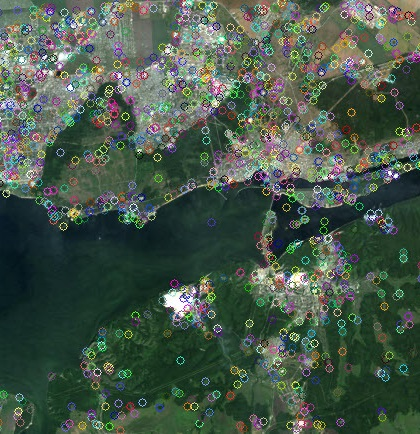
\includegraphics[width=0.45\textwidth,height=0.45\textwidth,]{keypoints/dam.jpg} 
		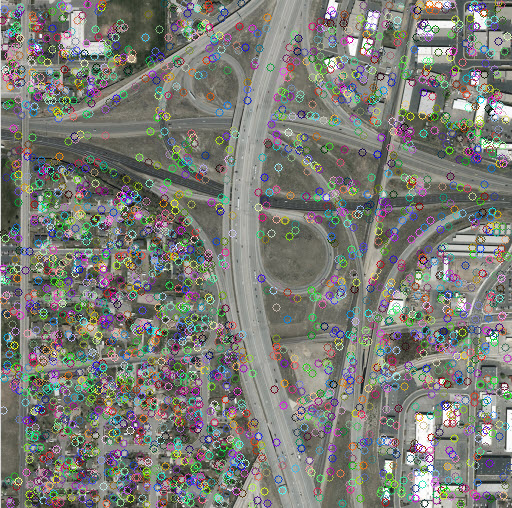
\includegraphics[width=0.45\textwidth,keepaspectratio]{keypoints/roads.jpg}                
		\centering\caption{ Пример наборов особых точек на фотографиях }
		\label{kps 1}                           
	\end{figure}    
	
	Для однозначного определения особой точки, инвариантного относительно ее координат в изображении, используются особые идентификаторы, называемые дескрипторами особых точек.
	Итак, алгоритм поиска должен обеспечивать вычисление достаточного набора дескрипторов особых точек, инвариантных к преобразованиям изображения, в первую очередь, пространственным. Далее будет дан общий обзор нескольких часто используемых на практике алгоритмов вычисления дескрипторов, реализации которых присутствуют в библиотеке компьютерного зрения OpenCV.
	
%	\begin{enumerate}[label=\arabic*)]%[label=\textbf{\arabic*}.]
		 {\bf Алгоритм SIFT} (Scale Invariant Feature Transform) был предложен Дэвидом Лоу в 2004 году [\ref{lowe surf}]. Дескрипторы SIFT устойчивы к изменению масштаба, аффинным преобразованиям и смене проекции исходных изображений. Алгоритм показал высокую эффективность, однако имеет высокую вычислительную сложность, что может являться проблемой при использовании его в режиме реального времени. SIFT включает как сам поиск точек, так и построение их дескрипторов.
		
		Алгоритм состоит из четырех основных шагов. На первом шаге производится выделение экстремумов изображения при помощи фильтра разности гауссианов (Difference of Gaussian). На втором шаге локализуются ключевые точки путем выявления наиболее контрастных областей. Далее, оценивается ориентация ключевых точек на основе локального градиента. На последнем этапе составляются дескрипторы, основанные на магнитуде и направлении градиента точек.
		
		\begin{figure}[H]
			\centering                             
			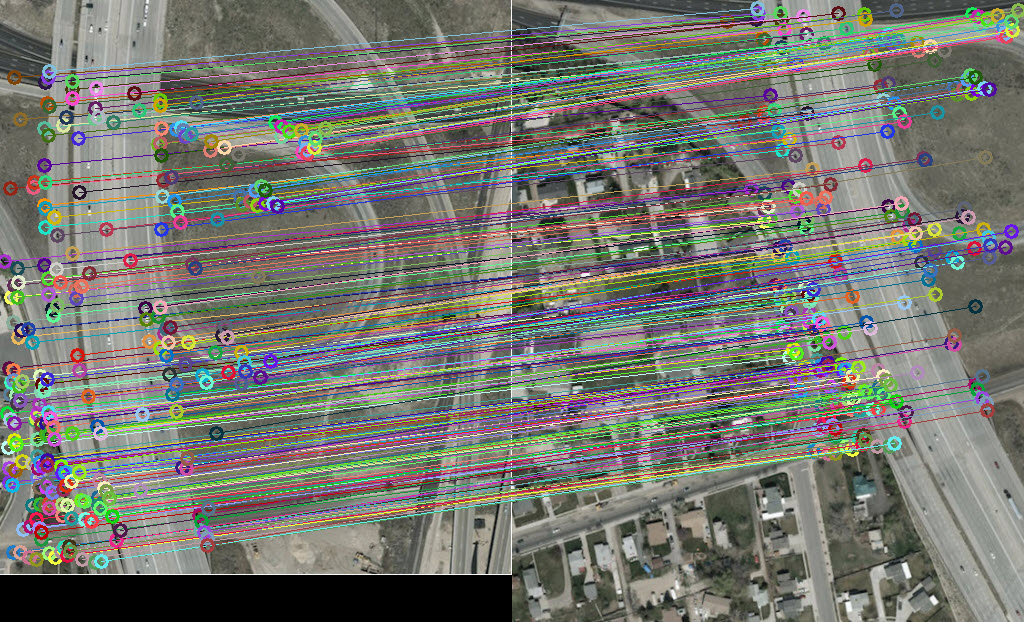
\includegraphics[width=0.5\textwidth,keepaspectratio]{descriptors/sift.jpg}                 
			\centering\caption{ Пример работы SIFT }
			\label{descriptors sift}                           
		\end{figure}    
		
		{\bf Алгоритм SURF} (Speeded up Robust Features) строит дескрипторы, инвариантные к изменению масштаба и вращения. SURF работает быстрее SIFT при незначительном снижении качества обнаружения.
		
		Для поиска экстремумов алгоритм аппроксимирует разность гауссианов матричными фильтрами, что позволяет увеличить производительность за счет высокой скорости самой операции свертки и легкости реализации параллельных вычислений. SURF использует детектор BLOB (Binary Large Objects) - крупных контрастных объектов [\ref{blobs}], основанный на матрице Гессе, для поиска ключевых точек.  Вычисление ориентации точек и построение дескрипторов основывается на вейвлет-образах (wavelet responses) окрестности точки.
		
		\begin{figure}[H]
			\centering                             
			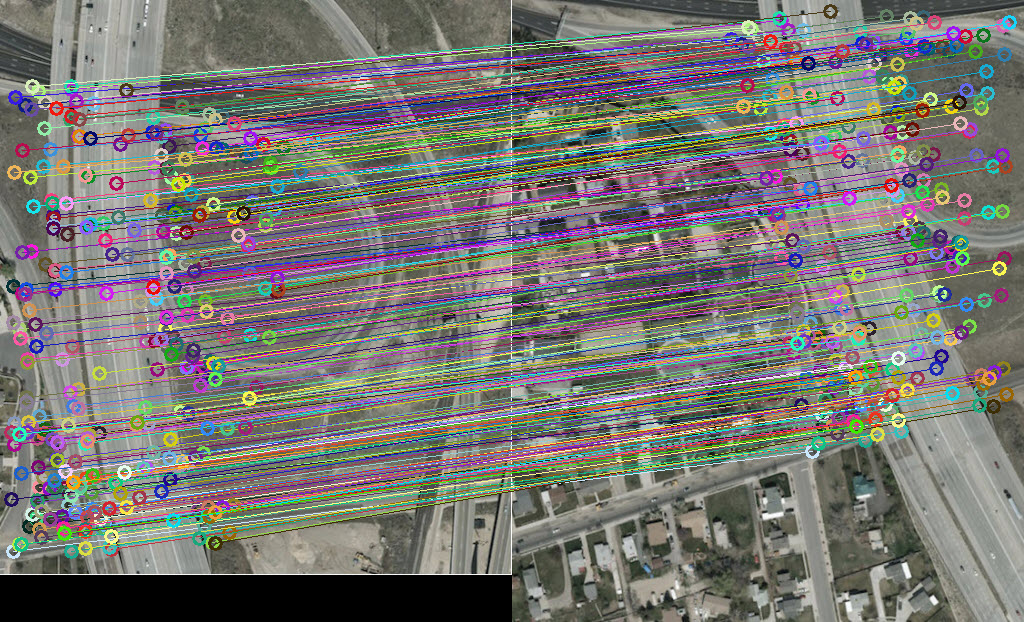
\includegraphics[width=0.5\textwidth,keepaspectratio]{descriptors/surf.jpg}                 
			\centering\caption{ Пример работы SURF }
			\label{descriptors surf}                           
		\end{figure}    
		
		{\bf Алгоритм ORB} (Oriented FAST and Rotated BRIEF) Эффективной альтернативной SIFT и SURF является ORB, комбинация детектора особых точек FAST и дескриптора BRIEF с некоторыми модификациями [\ref{rublee orb}]. 
		
		Первоначальный набор точек ищется с помощью FAST, после чего применяется детектор углов Харриса для нахождения наиболее интересных из них. FAST не вычисляет ориентацию точки, и, следовательно, не инвариентен к поворотам изображения. Для устранения этого фактора, для каждого найденного угла вычисляется точка наибольшей интенсивности в окрестности, и вектор из цетра угла до этой точки используется для описания ориентации. Некоторые дополнительные модификации позволяют получить достаточно инвариантные к преобразованиям дескрипторы точек. 
		
		\begin{figure}[H]
			\centering                             
			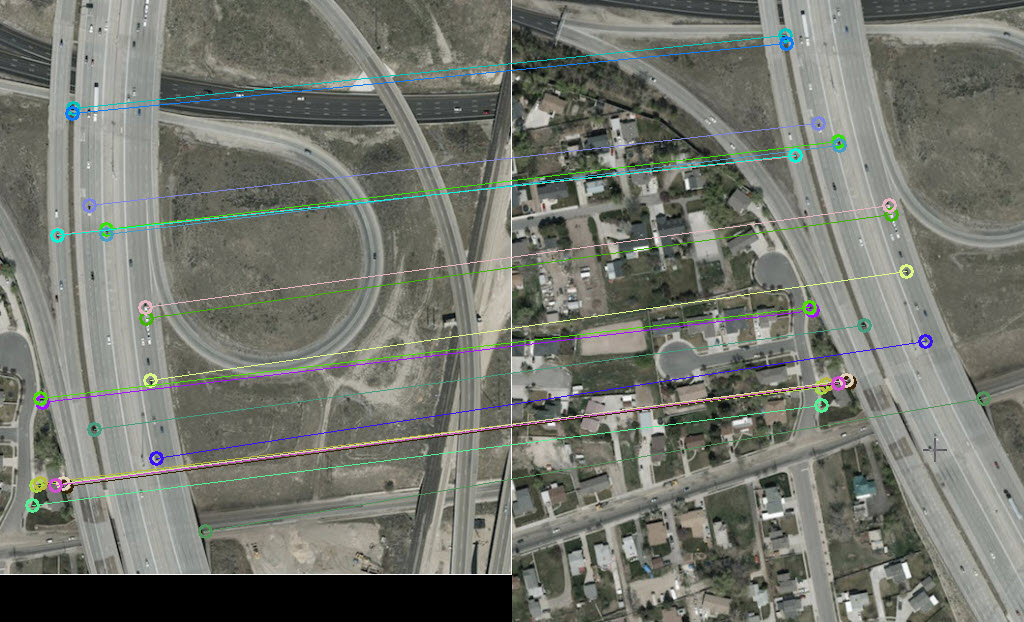
\includegraphics[width=0.5\textwidth,keepaspectratio]{descriptors/orb.jpg}                 
			\centering\caption{ Пример работы ORB }
			\label{descriptors orb}                           
		\end{figure}    
		
%	\end{enumerate}
}
\subsection{Пространственные преобразования изображений}{	
	Для работы с изображениями из существующих видов пространственных преобразований, как правило, используют три их группы: преобразования подобия, аффинные и проективные преобразования.
	
	Для рассмотрения и практического применения в данной работе наиболее интересными являются проективные преобразования, являющиеся общим случаем пространственных преобразований [\ref{wiki projective}]. Практическую ценность представляет то, что проективные преобразования позволяют бороться с перспективными искажениями - изменением масштаба объектов на фотографиях, возникающим, если снимаемые объекты находятся не плоскости, перпендикулярной направлению камеры, либо у края кадра при использовании широкого поля зрения.	
	
	Проективные преобразования отображают проекцию двумерного изображения на плоскость в трехмерном пространстве. Отличительной особенностью является сохранение коллинеарности точек, т.е. точки, лежавшие на одной прямой, после преобразования остаются на ней. Отличительной особенностью является несохранение параллельности прямых линий, а также изменение размера объектов в зависимости от расстояния от центра проекции.
	
	Преобразование над изображением $I$ задается как операция над каждым его пикселем с координатами $\begin{bmatrix}x&y\end{bmatrix}$, преобразующая данные координаты к $\begin{bmatrix}x'&y'\end{bmatrix}$. Изменение координат задается матрицей размерности 3х3 следующего вида:
	
	$$
	H = 
	\begin{bmatrix}
	h_{00} &\quad h_{01} &\quad h_{02} \\
	h_{10} &\quad h_{11} &\quad h_{12} \\
	h_{20} &\quad h_{21} &\quad h_{22} \\
	\end{bmatrix}.
	$$	
	\\
	
	Операция над координатами пикселей выполняется в виде умножения координатного вектора на матрицу преобразования. Очевидным образом, для работы с матрицей размерности 3х3, к координатному вектору положения точки $\begin{bmatrix}x&y\end{bmatrix}$ добавляется третья координата, равная 1 и не влияющая на результат.
	
	$$
	\begin{bmatrix}x'\\y'\\1\end{bmatrix} = 
	H\begin{bmatrix}x\\y\\1\end{bmatrix} = 
	\begin{bmatrix}
	h_{00} &\quad h_{01} &\quad h_{02} \\
	h_{10} &\quad h_{11} &\quad h_{12} \\
	h_{20} &\quad h_{21} &\quad h_{22} \\
	\end{bmatrix}
	\begin{bmatrix}x\\y\\1\end{bmatrix}.
	$$\\
	
	
	В соответствии с правилами матричного умножения, координаты пикселей вычисляются по следующим формулам:
	\begin{equation}\label{coordinates}
	x' = h_{00}x + h_{01}y + h_{02},\\
	y' = h_{10}x + h_{11}y + h_{12}.
	\end{equation}	
	
	Отметим, что использование в качестве матрицы преобразования единичной матрицы размерности 3х3 оставляет исходное изображение без изменений. На рисунке \ref{projectivе transform} приведен пример проективных преобразований изображения.
	
	\begin{figure}[H]
		\centering                             
		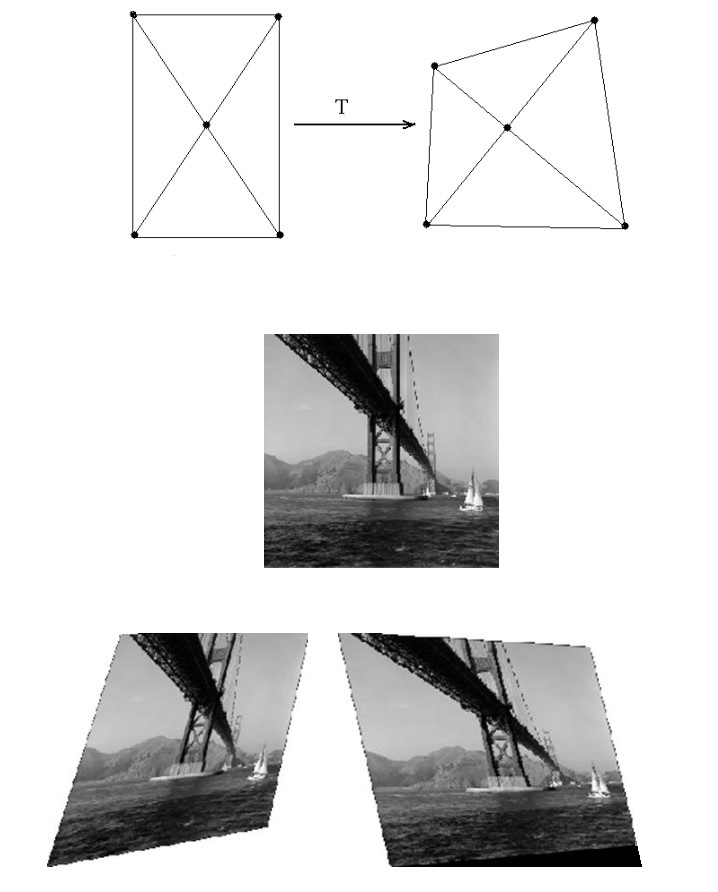
\includegraphics[width=0.4\textwidth,keepaspectratio]{transforms/projection.jpg}                 
		\centering\caption{ Пример проективных преобразований }
		\label{projectivе transform}                           
	\end{figure}    

	Подмножеством проективных преобразований являются аффинные преобразования. Их отличительной чертой выступает сохранение параллельности линий на изображении [\ref{wiki affine}]. При помощи аффинных преобразований выполняется смещение, поворот и масштабирование. 
	
	Операция смещения на $e$ по оси $x$ и на $f$ по оси $y$ задается следующей матрицей преобразования:
	$$
	H_t = 
	\begin{bmatrix}
	1 &\quad 0 &\quad 0 \\
	0 &\quad 1 &\quad 0 \\
	e &\quad f &\quad 1 \\
	\end{bmatrix}.
	$$
	Операция поворота на угол $\alpha$ задается матрицей поворота:
	$$
	H_r = 
	\begin{bmatrix}
	\cos(\alpha) &\quad \sin(\alpha) &\quad 0 \\
	-\sin(\alpha) &\quad \cos(\alpha) &\quad 0 \\
	0 &\quad 0 &\quad 1 \\
	\end{bmatrix}.
	$$
	Операция масштабирования с коэффициентом $a$ по оси $x$ и $d$ по оси $y$ задается следующей матрицей:
	$$
	H_s = 
	\begin{bmatrix}
	a &\quad 0 &\quad 0 \\
	0 &\quad d &\quad 0 \\
	0 &\quad 0 &\quad 1 \\
	\end{bmatrix}.
	$$  		
	
	
	Рассмотрим нахождение пространственного преобразования по опорным точкам.
	Напомним, что система уравнений, описывающих его, записана в выражении \eqref{coordinates}.
%	$$
%	x' = h_{00}x + h_{01}y + h_{02},$$ $$
%	y' = h_{10}x + h_{11}y + h_{12}.	
%	$$	
	Приведем пример вычисления коэффициентов матрицы $h_{00} \hdots h_{12}$ для простейшего случая с использованием минимально необходимых трех пар соответствующих ключевых точек.
	Система соответствующих уравнений в матричной форме запишется как:	
	$$
	\begin{bmatrix}
	x'_1 \\ x'_2 \\ x'_3
	\end{bmatrix}
	= A
	\begin{bmatrix}
	h_00 \\ h_01 \\ h_02
	\end{bmatrix},
	$$
	$$
	\begin{bmatrix}
	y'_1 \\ y'_2 \\ y'_3
	\end{bmatrix}
	= A
	\begin{bmatrix}
	h_10 \\ h_11 \\ h_12
	\end{bmatrix}.
	$$
	\begin{tabular}{ rl }
		\qquad где 
		& $A$ - матрица следующего вида:\\
		& $A = 
		\begin{bmatrix}
		1 & x_1 & y_1 \\
		1 & x_2 & y_2 \\
		1 & x_3 & y_3 \\
		\end{bmatrix}.$ \\
	\end{tabular}\newline
	
	
	Для получения значений коэффициентов домножим каждую часть обоих систем на обратную матрицу $A^{-1}$. Таким образом, получим следующие выражения для вычисления коэффициентов в матричной форме:
	$$
	\begin{bmatrix}
	h_00 \\ h_01 \\ h_02
	\end{bmatrix}
	= A^{-1}
	\begin{bmatrix}
	x'_1 \\ x'_2 \\ x'_3
	\end{bmatrix},
	$$
	$$
	\begin{bmatrix}
	h_10 \\ h_11 \\ h_12
	\end{bmatrix}
	= A^{-1}
	\begin{bmatrix}
	y'_1 \\ y'_2 \\ y'_3
	\end{bmatrix}.
	$$
	
	
	Вычисленный набор коэффициентов подставляется в выражение преобразования и используется для произведения операции с каждым пикселем исходного изображения.
	При использовании большего числа пар опорных точек, чем три, значения усредняются, что позволяет уменьшить неизбежно возникающие на практике погрешности.
}
}
\newpage

\section{Модели цифровых шумов в обработке изображений}
{
	Цифровым шумом изображения называют дефекты, вносимые в изображение спецификой конструкции и несовершенством цифровых фотосенсоров, электроники фото- и видеотехники, их использующей, а также фотонной природой света. 
	Цифровой шум визуально проявляется отдельными элементами изображения, имеющими размеры в один или несколько пикселей, отличающимися от основного изображения своей яркостью (яркостной шум, luminance noise) и (или) цветом (chrominance noise, хроматический шум). 
	
	По способу влияния на изображение цифровые шумы разделяются на три группы:
	\begin{enumerate}%[label=\arabic*)]
		\item Аддитивные -- значение шума складывается со значением сигнала. Производят пиксели изображения, отличающиеся по яркости и (или) цвету от исходного на некоторое значение. Величина шума не зависит от величины сигнала.
		\item Мультипликативные -- значение шума умножается на значение сигнала. Производят пиксели изображения, отличающиеся по яркости и (или) цвету от исходного на определенную долю. Величина шума зависит от величины сигнала.
		\item Импульсные -- замещают случайные пиксели исходного изображения точками со значительными скачками яркости и (или) цвета. Величина шума от величины сигнала не зависит.
	\end{enumerate}
	
	Рассмотрим несколько математических моделей цифрового шума, стандартно используемых для оценки качества алгоритмов обработки изображений.\\
	
%	\begin{enumerate}[label=\arabic*)]%[label=\textbf{\arabic*}.]
	{\bf Гауссовский шум} -- случайный аддитивный шум с независимыми значениями для каждого пикселя, не зависящий от их исходной яркости. Плотность распределения вероятности гауссовского шума задается нормальным распределением:
	$$p_G(z)=\dfrac{1}{\sigma\sqrt{2\pi}}{\rm e}^{-\dfrac{(z-\mu)^2}{2\sigma^2}},$$
	\begin{tabular}{ rl }
		где 
		& $z$ -- яркость пикселя;\\
		& $\mu$ -- среднее значение распределения; \\
		& $\sigma$ -- среднеквадратичное отклонение. \\
	\end{tabular}\\

	Гауссовский шум используется в качестве стандарта белого шума при тестировании цифрового оборудования и алгоритмов.	Применительно к фотографиям данная модель шума имитирует помехи, возникающие при недостаточной освещенности или экспозиции. Пример представлен на рисунках \ref{noises_gauss} - \ref{noises_gauss_big}.
 
	\begin{figure}[H]
		\centering                             
		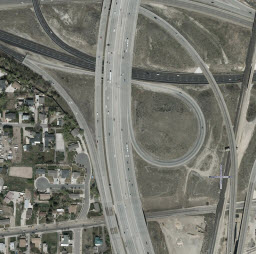
\includegraphics[width=0.35\textwidth,keepaspectratio]{noises/original.jpg}   
		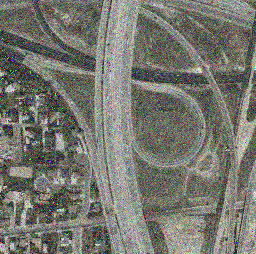
\includegraphics[width=0.35\textwidth,keepaspectratio]{noises/gauss.jpg}                 
		\centering\caption{ Пример гауссовского шума с $\sigma=30$ }
		\label{noises_gauss}                           
	\end{figure}    

	\begin{figure}[H]
		\centering                             
		
\includegraphics[width=0.35\textwidth,keepaspectratio]{noises/gauss_big.jpg}                   
		\centering\caption{ Участок изображения при увеличении }
		\label{noises_gauss_big}                           
	\end{figure}    
	
	 {\bf Шум соль-перец} -- случайный импульсный шум c независимыми значениями для каждого пикселя. Характеризуется случайно распределенными по изображению точками черного и белого цвета. В данной работе использовалась реализация с одним параметром вероятности возникновения шума $p$ и определением черного или белого цвета с вероятностями $p$ и $1-p$ соответственно. Пример представлен на рисунках \ref{noises sp} - \ref{noises sp big}.
	 
	\begin{figure}[H]
		\centering                             
		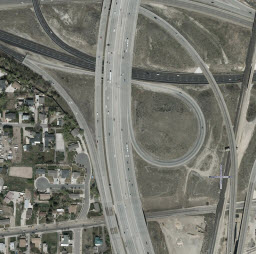
\includegraphics[width=0.35\textwidth,keepaspectratio]{noises/original.jpg}   
		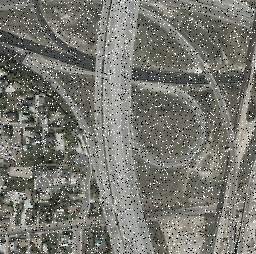
\includegraphics[width=0.35\textwidth,keepaspectratio]{noises/sp.jpg}                 
		\centering\caption{ Пример шума соль-перец с $p=0{,}05$ }
		\label{noises sp}                           
	\end{figure}    

	\begin{figure}[H]
		\centering                             
		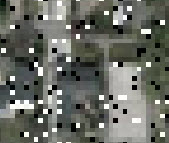
\includegraphics[width=0.35\textwidth,keepaspectratio]{noises/sp_big.jpg}                   
		\centering\caption{ Участок изображения при увеличении }
		\label{noises sp big}                           
	\end{figure}    
	
%	\item {\bf Мультипликативный шум}
%	\begin{figure}[H]
%		\centering                             
%		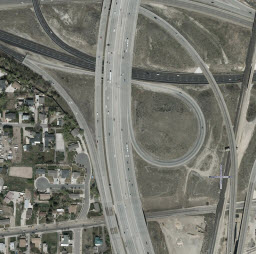
\includegraphics[width=0.35\textwidth,keepaspectratio]{noises/original.jpg}   
%		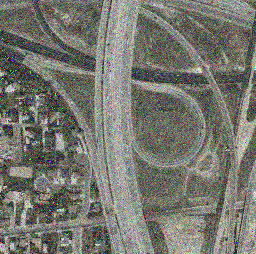
\includegraphics[width=0.35\textwidth,keepaspectratio]{noises/gauss.jpg}                 
%		\centering\caption{ Пример проективных преобразований }
%		\label{noises speckle}                           
%	\end{figure}    
	
	\newpage
	 {\bf Размытие} -- строго говоря, не являясь цифровым шумом, представляет собой часто встречающийся дефект изображения, возникающий из-за неправильной фокусировки. В данной работе размытие интересно тем, что обладает свойством сглаживать высокочастотные компоненты изображения (мелкие детали), серьезно влияя на определение особых точек. Также, размытие является статичным процессом без использования случайных значений, что позволяет легко воспроизводить результаты. На практике, как правило, используется реализация размытия в виде фильтра Гаусса -- матричного фильтра, усредняющего значений соседних пикселей в соответствии с нормальным распределением. Формула размытия является двумерной функцией Гаусса:
	$$G(x, y)=\dfrac{1}{2\pi\sigma^2}{\rm e}^{-\dfrac{x^2+y^2}{2\sigma^2}},$$
	\begin{tabular}{ rl }
		где 
		& $x, y$ -- расстояния по осям от центра;\\
		& $\sigma$ -- среднеквадратичное отклонение. \\
	\end{tabular}\\

	Пример представлен на рисунках \ref{noises blur} - \ref{noises blur big}.
	\begin{figure}[H]
		\centering                             
		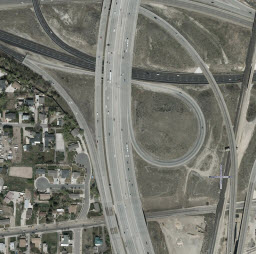
\includegraphics[width=0.35\textwidth,keepaspectratio]{noises/original.jpg}   
		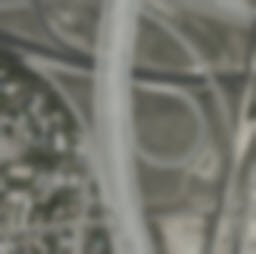
\includegraphics[width=0.35\textwidth,keepaspectratio]{noises/blur.jpg}                 
		\centering\caption{ Пример размытия изображения с $m=21$ }
		\label{noises blur}                           
	\end{figure}    
		\begin{figure}[H]
		\centering                             
		
\includegraphics[width=0.35\textwidth,keepaspectratio]{noises/blur_big.jpg}                   
		\centering\caption{ Участок изображения при увеличении }
		\label{noises blur big}                           
	\end{figure}    
%	\end{enumerate}	

	Как было сказано ранее, дескрипторы при поиске особых точек определяются как функции от яркости определенной окрестности пикселя. Зная это, можно понять, что зашумленность изображения будет вызывать сбои при вычислении дескрипторов, приводя к уменьшению количества найденных совпадений, или к искажению координат точек. В предельном случае, когда необходимое для построения матрицы проективного преобразования количество особых точек не может быть найдено, высокая зашумленность изображения полностью блокирует работу алгоритма. В остальных случаях ошибки в вычисленных дескрипторах будут приводить к смещению изображения относительно требуемого после трансформации положения, и, соответственно, к визуально заметным неточностям.
}
\newpage

\section{Экспериментальное исследование}
{
   	\subsection{Реализация алгоритма сшивки}{
   		
   		Алгоритм сшивки изображений для исследования был реализован на языке Python 3.7 с использованием библиотеки OpenCV 3.4.2. 
   		
   		Функция, осуществляющая процедуру совмещения, принимает на вход два изображения и тип используемого дескриптора. 
   		Используются дескрипторы SIFT, SURF, ORB, BRIEF. Заметим, что алгоритмы SIFT и SURF являются патентованными, и не присутствуют в стандартной библиотеке OpenCV из-за лицензионных ограничений. Данные алгоритмы доступны в пакете xfeatures2d при использовании версии библиотеки, включающей неофициальные алгоритмы, opencv-contrib. Использование данных алгоритмов разрешается только в некоммерческих целях [\ref{cv docs}]. 
   		
   		Для вычисления дескрипторов производится преобразование исходных изображений в градации серого.
   		
   		\begin{lstlisting}[frame=single,language=Python,mathescape=true] 
   		# convert the image to grayscale
   		gray = cv2.cvtColor(image, cv2.COLOR_BGR2GRAY)
   		\end{lstlisting}
   		
   		Производится поиск наборов особых точек при помощи выбранного дескриптора.
   	
   		\begin{lstlisting}[frame=single,language=Python,mathescape=true] 
   		# detect keypoints in the image
   		detector = cv2.FeatureDetector_create("SIFT")
   		kps = detector.detect(gray)
   		
   		# extract features from the image
   		extractor = cv2.DescriptorExtractor_create("SIFT")
   		(kps, features) = extractor.compute(gray, kps)
   		\end{lstlisting}
   		
   		Найденные наборы проверяются на совпадение дескрипторов методом knn. Полученные совпадения дополнпительно тестируются на предмет нахождения расстояния между точками в заданных пределах. Пары, прошедшие тест, используются для вычисления преобразования.
   		
   		\begin{lstlisting}[frame=single,language=Python,mathescape=true] 
   		# compute the raw matches and initialize the list of actual
   		# matches
   		matcher = cv2.DescriptorMatcher_create("BruteForce")
   		rawMatches = matcher.knnMatch(featuresA, featuresB, 2)
   		matches = []
   		
   		# loop over the raw matches
   		for m in rawMatches:
   		# ensure the distance is within a certain ratio of each
   		# other (i.e. Lowe's ratio test)
   		if len(m) == 2 and m[0].distance < m[1].distance * ratio:
   		matches.append((m[0].trainIdx, m[0].queryIdx))
   		\end{lstlisting}
   		
   		После нахождения совпавших точек, по их наборам для каждого изображения вычисляется матрица проективного преобразования.
   		Если совпавших опорных точек найдено меньше, чем четыре, проективное преобразование не может быть вычислено, и функция возвращает статус ошибки.
   		
   		\begin{lstlisting}[frame=single,language=Python,mathescape=true]
   		 # compute the homography between the two sets of points
   		(H, status) = cv2.findHomography(ptsA, ptsB, cv2.RANSAC,
   		reprojThresh)
   		\end{lstlisting}
   		
   		Построенная матрица проективного преобразования применяется ко второму входному изображению, трансформируя его до совпадения положений опорных точек.
   		
   		Исходное первое изображение и преобразованное второе записываются в одно результирующее. В зависимости от требуемых параметров, сложение может производиться с различными значениями альфа-канала, в том числе с выделением яркостью пересекающейся области либо одного из изображений в целях повышения наглядности.
   		
   		Функция возвращает результирующее изображение и отчет о работе алгоритма, включающий время выполнения и построенную матрицу проективного преобразования.
   		
   		Полный код функции представлен в приложении А.
   	}
   
   	\newpage
   	\subsection*{3.2 \quad Экспериментальная оценка влияния цифровых шумов на \\ качество работы алгоритма}{
   		\addcontentsline{toc}{subsection}{3.2\qquad Экспериментальная оценка влияния цифровых шумов на качество работы алгоритма}
   		Выбранные для исследования цифровые шумы реализованы в виде отдельных функций, принимающих на вход изображение, подлежащее зашумлению, и параметры шума. Исходный код функций зашумления представлен в приложении А.
   		
   		В качестве оценочных параметров точности работы алгоритма были выбраны общее количество найденных особых точек, процент совпадений от общего числа и смещение преобразованного изображения относительно истинного положения в результате неточности построенной матрицы проективного преобразования.
   		Количество найденных точек возвращается функцией сшивки после успешного завершения работы. Смещение относительно истинного положения вычисляется по координатам углов исходного и преобразованного изображений, оценочными параметрами смещения выступают медиана и максимум расстояний между соответствующими углами в пикселях. 
   		
   		Результаты экспериментов сохраняются в виде текстовых отчетов и (или) изображений, доступных для дальнейшего анализа и визуализации.
   		
   		Для приведенных экспериментов вторым изображением, поступающим на вход алгоритма сшивки, выступала программно вырезанная прямоугольная часть центральной области первого изображения, равная 25 процентам его площади. Такой подход, в отличии от аналогичного практическому применению алгоритма использования частично пересекающихся фотографий, позволяет гарантировать нахождение максимального принципиально возможного количества совпадающих точек, а также упростить расчет смещения и визуализацию.
   		\newpage
%   		\begin{enumerate}[label=\arabic*)]%[label=\textbf{\arabic*}.]
   			\subsubsection{ Сравнение работы алгоритмов при применении размытия } Размытие изображения, строго говоря, не является цифровым шумом, хотя и может быть достаточно распространенным дефектом фотографии. Тем не менее, размытие хорошо подходит для общего сравнения алгоритмов, так как является стационарным и легко воспроизводимым процессом понижения качества картинки. 
   			
   			В данном эксперименте входное изображение размывалось с итеративным увеличением размера ядра гауссовского фильтра $m$. Эксперимент прекращался, когда число найденных опорных точек становилось меньше четырех. Входные изображения приводились к размеру в 512 пикселей по горизонтали. На рисунках \ref{blur_sample 1}-\ref{blur sample 2} представлены примеры результатов работы программы.
   			
   			\newpage
   			\begin{figure}[H]
   				\centering                             
   				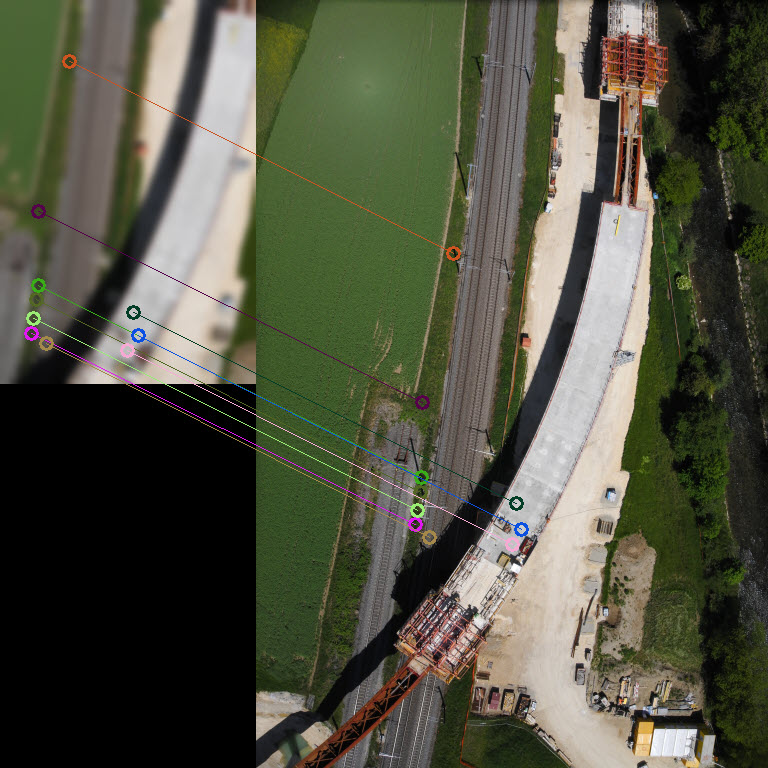
\includegraphics[width=0.65\textwidth,keepaspectratio]{samples/blur_matches.jpg}   
   				\centering\caption{ Пример отображения программой совпадений особых точек на размытом изображении }
   				\label{blur_sample 1}                           
   			\end{figure}    
   		
	   		\begin{figure}[H]
	   			\centering                                
	   			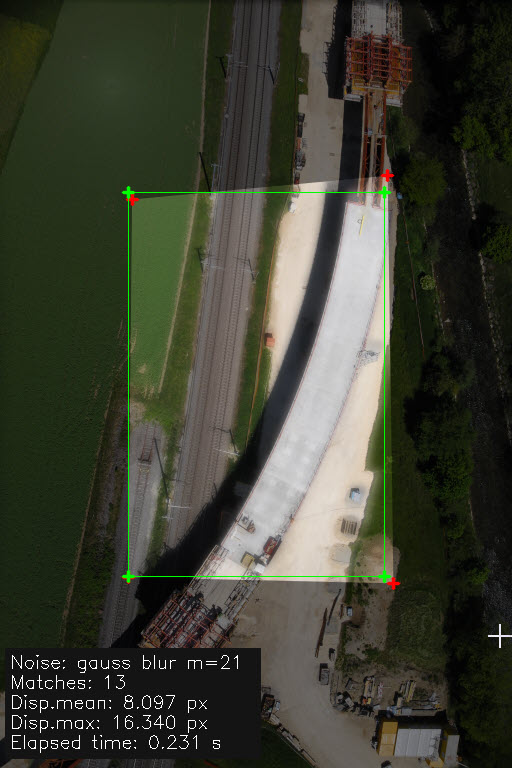
\includegraphics[width=0.45\textwidth,keepaspectratio]{samples/blur_result.jpg}       
	   			\centering\caption{ Пример отображения программой результата совмещения}
	   			\label{blur sample 2}                           
	   		\end{figure}    
   			\newpage
   			
   			\begin{table}[H]                               
   				\centering                                  
   				\caption{ Сравнение числа найденных точек при увеличении уровня размытия }                            
   				\begin{tabularx}{\textwidth}{ | c | Y | Y | Y | }
   					\hline                     
   					\multirow{2}{*}{m} & \multicolumn{3}{c}{Алгоритмы} \vline \\ \cline{2-4} 
   					&     SIFT &  SURF &  ORB  \\ \hline                           
   					- &  496  &  996 & 1286 \\ \hline
					3 &  276  &  481 & 685 \\ \hline   		
					7 &  93  &  187 & 237 \\ \hline 
					11 &  51  &  87 & 106 \\ \hline  
					17 &  25  &  48 & 23 \\ \hline 	
					19 &  21  &  42 & 17 \\ \hline 			
					21 &  16  &  30 & 9 \\ \hline 
					27 &  9  &  22 & - \\ \hline
					35 &  6  &  16 & - \\ \hline
					41 &  7  &  8 & - \\ \hline	
					49 &  5  &  6 & - \\ \hline	
					53 &  5  &  - & - \\ \hline			
   				\end{tabularx}
   				\label{ex1_count}                                
   			\end{table}           
   		
   			Прочерком обозначены значения, при которых алгоритм находит менее четырех совпадающих опорных точек.
   		
   			\begin{table}[H]                               
   				\centering                                  
   				\caption{ Сравнение медианы смещения при увеличении уровня размытия }                            
   				\begin{tabularx}{\textwidth}{ | c | Y | Y | Y | }
   					\hline                     
   					\multirow{2}{*}{m} & \multicolumn{3}{c}{Алгоритмы} \vline \\ \cline{2-4} 
   					&   SIFT &  SURF &  ORB  \\ \hline                           
   					- &  0,032  &  0,000 & 0,130 \\ \hline
   					3 &  0,082  &  0,085 & 0,163 \\ \hline
   					7 &  0,146  &  0,170 & 2,670 \\ \hline
   					11 &  0,270  &  0,303 & 1,953 \\ \hline
   					17 &  0,917  &  1,100 & 2,852 \\ \hline
   					19 &  0,405  &  1,476 & \cellcolor{blue!25} 15,543 \\ \hline
   					21 &  2,243  &  2,893 & \cellcolor{blue!25} 336,972 \\ \hline 	
   					27 &  5,564  &  1,012 & \cellcolor{blue!25} - \\ \hline		
   					35 & \cellcolor{blue!25} 13,711  &  5,951 & \cellcolor{blue!25} - \\ \hline	
   					41 & \cellcolor{blue!25} 44,210  & \cellcolor{blue!25} 10,701 & \cellcolor{blue!25} - \\ \hline
   					49 & \cellcolor{blue!25} 84,046  & \cellcolor{blue!25} 22,116 & \cellcolor{blue!25} - \\ \hline	
   					53 & \cellcolor{blue!25} 120,100  & \cellcolor{blue!25} - & \cellcolor{blue!25} - \\ \hline	
   				\end{tabularx}
   				\label{ex1 disp}                                
   			\end{table}       
   		
   			В таблице \ref{ex1 disp} цветом выделены значения медианы смещения в более чем 10 пикселей, как выбранный критерий хорошо различимого визуально показателя недостаточной точности. Прочерком обозначены значения, при которых алгоритм находит менее четырех совпадающих опорных точек.
   			
   			Результаты эксперимента отражены на рисунке \ref{blur_mch_disp}.
   			
   			\begin{figure}[H]
   				\centering                             
   				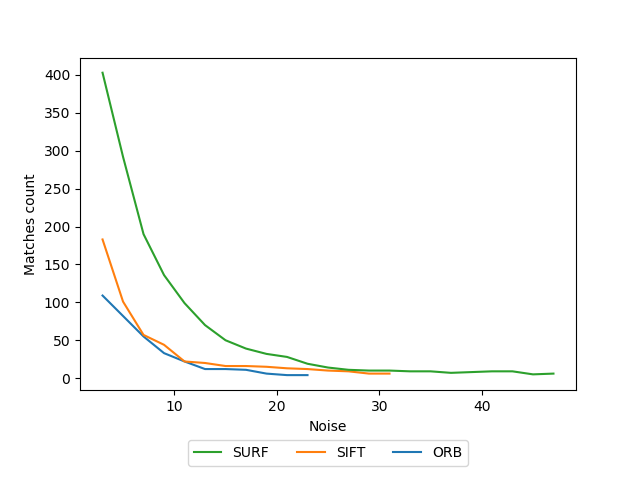
\includegraphics[width=0.75\textwidth,keepaspectratio]{ex1/Rand_noises_matches.png}   
   				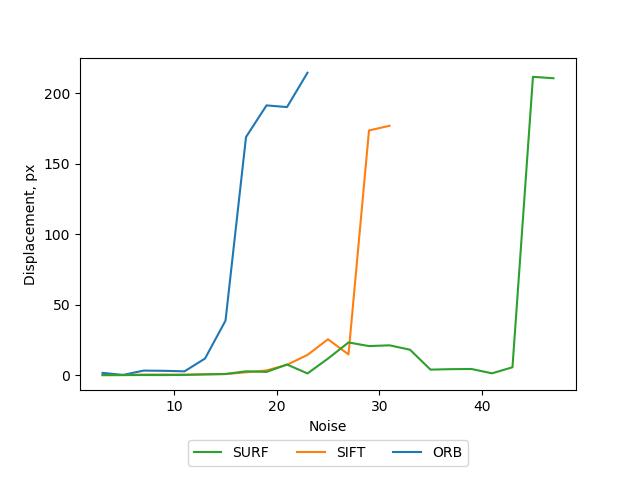
\includegraphics[width=0.75\textwidth,keepaspectratio]{ex1/Rand_noises_displacement.png}       
   				\centering\caption{ Поведение числа совпадений точек и смещения при размытии изображения }
   				\label{blur_mch_disp}                           
   			\end{figure}    
   			
   			\newpage
   			\subsubsection{ Сравнение работы алгоритмов при применении случайных шумов } При использовании случайных шумов эксперимент производился несколько раз для каждого уровня зашумленности с усреднением результатов для устранения флуктуаций и получения более общей картины. 
   			
   			Для каждого уровня зашумленности значения усреднялись по 30 экспериментам. Варьируемыми параметрами шумов выступали стандартное отклонение $\sigma$ для гауссовского шума и вероятность $p$ для шума соль-и-перец. Эксперимент прекращался, когда число найденных опорных точек становилось меньше четырех. Входные изображения приводились к размеру в 512 пикселей по горизонтали.
   			
   			Результаты экспериментов отражены на рисунках \ref{rand_noises_gauss}-\ref{rand_noises_sp}. 
   			
   			\begin{figure}[H]
   				\centering                             
   				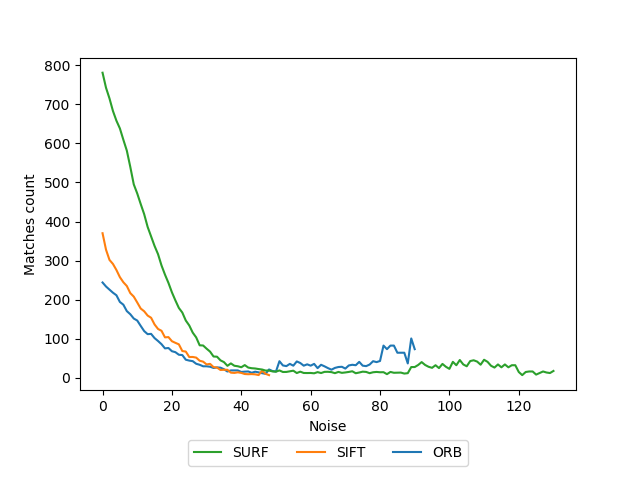
\includegraphics[width=0.75\textwidth,keepaspectratio]{ex2/gauss/Rand_noises_matches.png}   
   				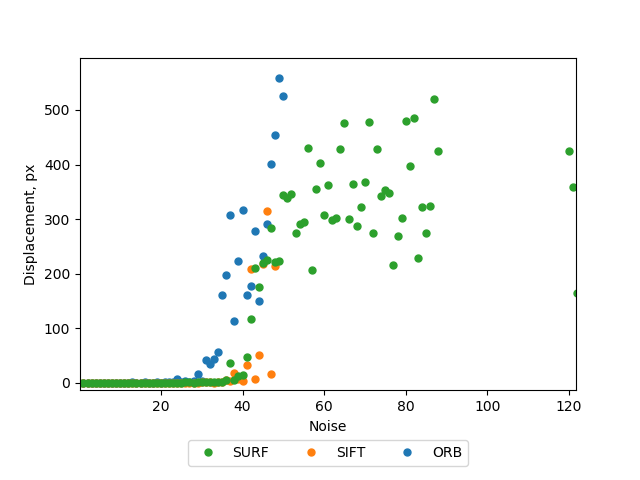
\includegraphics[width=0.75\textwidth,keepaspectratio]{ex2/gauss/Rand_noises_displacement.png}       
   				\centering\caption{ Поведение числа совпадений точек и смещения при использовании гауссовского шума }
   				\label{rand_noises_gauss}                           
   			\end{figure}    
   		
   			\begin{figure}[H]
   				\centering                             
   				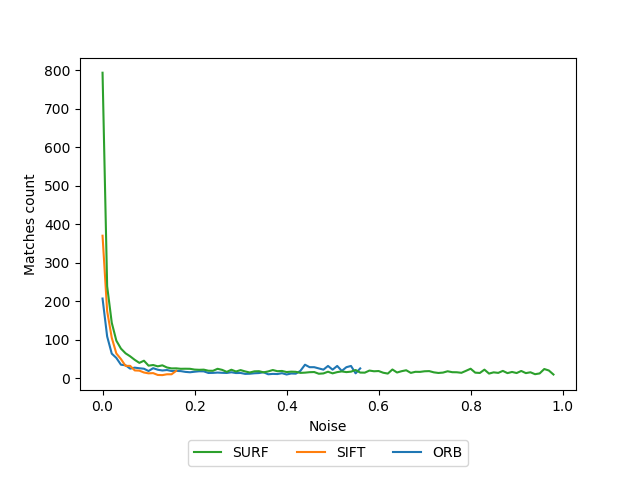
\includegraphics[width=0.75\textwidth,keepaspectratio]{ex2/sp/Rand_noises_matches.png}   
   				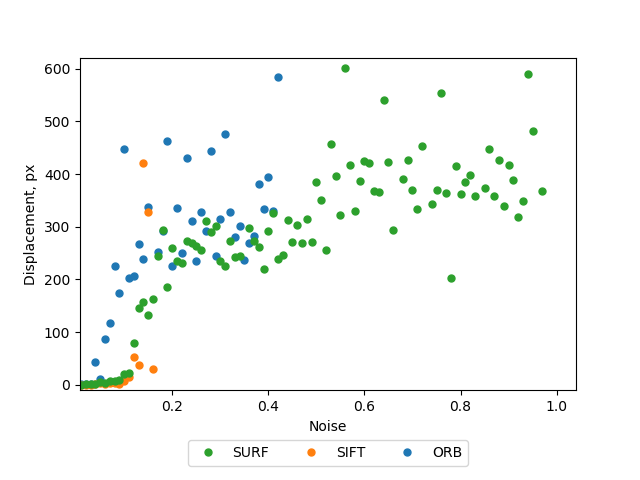
\includegraphics[width=0.75\textwidth,keepaspectratio]{ex2/sp/Rand_noises_displacement.png}       
   				\centering\caption{ Поведение числа совпадений точек и смещения при использовании шума соль-и-перец}
   				\label{rand_noises_sp}                           
   			\end{figure}   
   			
%   		\end{enumerate}	
}
}

\newpage
\section{Анализ полученных результатов}
{
    Проанализируем полученные результаты. Эксперименты показывают несколько интересных факторов в работе алгоритмов. 
    
    При размытии изображения дескриптор ORB раньше других рассмотренных начинает терять точность, несмотря на значительно большее общее количество найденных совпадений. Серьезное искажение результата достигается при размерах ядра Гауссова фильтра более 17 для тестового изображения размером 512 на 512 пикселей, с дальнейшим увеличением размера ядра ORB первым перестает находить достаточное число точек. Наилучшим образом при работе с размытым изображением показывает себя дескриптор SURF.
    
    У всех рассмотренных алгоритмов наблюдается резкое увеличение искажения результата при переходе определенного порогового значения размытия.
    
    На графике \ref{blur d by m} можно наблюдать резкое падение качества при числе точек, меньшем чем 20. Это объясняется тем, что размытие может сильно ухудшать точность определения координат особых точек, даже при сохранении общей яркостной картины достаточном для построения дескриптора. Соответственно, при малых количествах точек, ошибки в отдельных координатах сильно влияют на построенную матрицу преобразования.
    
    \begin{figure}[H]
    	\centering                             
    	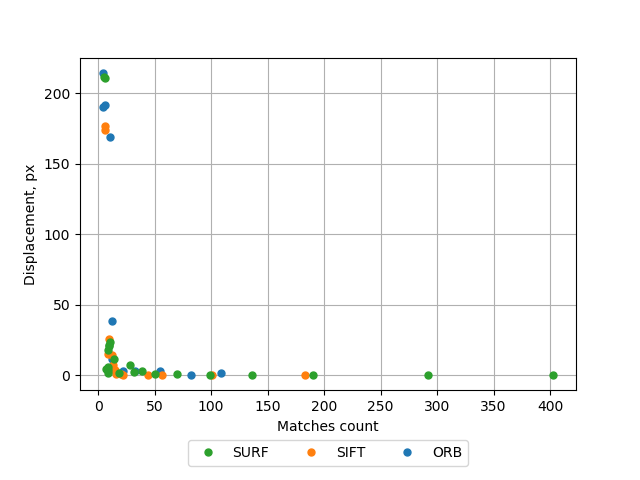
\includegraphics[width=0.75\textwidth,keepaspectratio]{ex1/Rand_noises_d_by_m.png}      
    	\centering\caption{  Изменение смещения с ростом числа точек при использовании размытия}
    	\label{blur d by m}    
	\end{figure} 
	
	При применении случайных шумов можно наблюдать более интересную картину. При использовании дескриптора SIFT точность падает равномерно, алгоритм перестает работать на тестовых изображениях при значении $\sigma$ гауссовского шума более 50 и при вероятности шума соль-перец более 0.15. При этом, остальные дескрипторы продолжают работать при значительно большем зашумлении, но стремительно теряют в точности, приводя к абсолютно непригодным для практического применения результатам. На рисунке \ref{fail surf} приведен пример результата, выданного алгоритмом SURF на значениях, при которых SIFT перестает работать. 
	
	\begin{figure}[H]
		\centering                             
		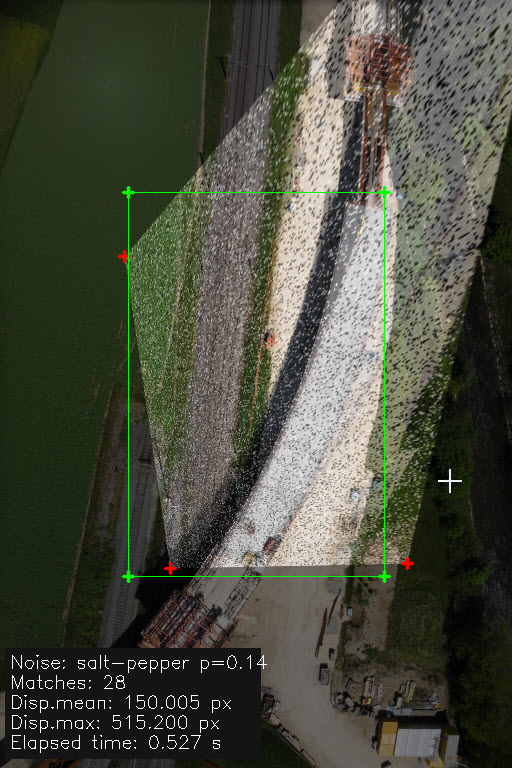
\includegraphics[width=0.45\textwidth,keepaspectratio]{fails/result.jpg}      
		\centering\caption{Пример искажения при использовании алгоритма SURF}
		\label{fail surf}    
	\end{figure} 

	Принимая во внимание практическую непригодность изображений с подобными уровнями шумов и искажений, можно отбросить диапазоны значений за пределами стабильной работы алгоритма SIFT. На графиках \ref{gauss disp big}-\ref{sp disp big} можно наблюдать этот диапазон. 
	
	\begin{figure}[H]
		\centering                             
		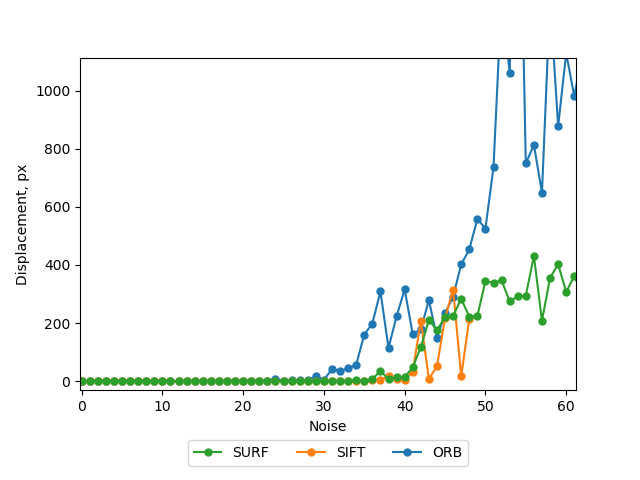
\includegraphics[width=0.60\textwidth,keepaspectratio]{ex2/gauss/Rand_noises_displacement_big.png}   
		\centering\caption{ Увеличенный фрагмент графика смещения при использовании гауссовского шума }
		\label{gauss disp big}                           
	\end{figure}    

	\begin{figure}[H]
		\centering                             
		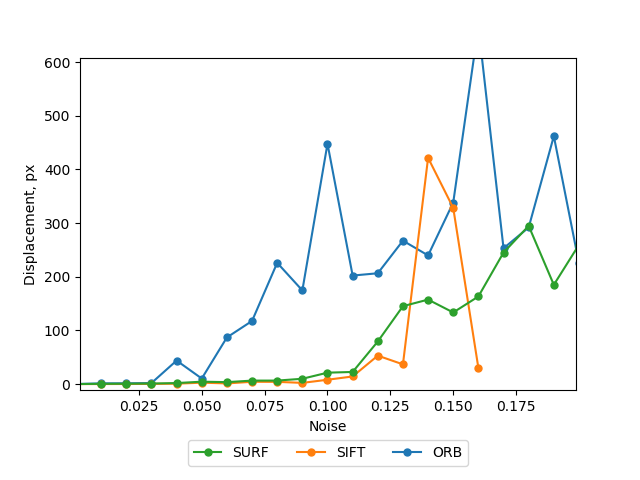
\includegraphics[width=0.60\textwidth,keepaspectratio]{ex2/sp/Rand_noises_displacement_big.png}       
		\centering\caption{ Увеличенный фрагмент графика смещения при использовании шума соль-перец }
		\label{sp disp big}                           
	\end{figure}    
	
	Как можно видеть, все три алгоритма сохраняют достаточную точность при практически достижимых уровнях гауссовского шума. Однако, ORB наименее устойчив к шуму соль-и-перец, что можно видеть по резкому пику на графике при вероятности 0.03, сохраняющемуся даже при усреднении по набору экспериментов.
	
	\begin{figure}[H]
		\centering                             
		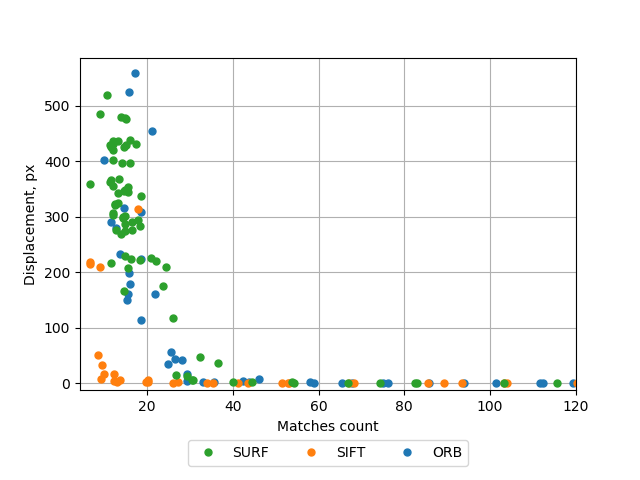
\includegraphics[width=0.6\textwidth,keepaspectratio]{ex2/gauss/Rand_noises_d_by_m.png}      
		\centering\caption{ Изменение смещения с ростом числа точек при использовании гауссовского шума}
		\label{rand_noises_gauss_b_by_m}                           
	\end{figure} 
	
	\begin{figure}[H]
		\centering                             
		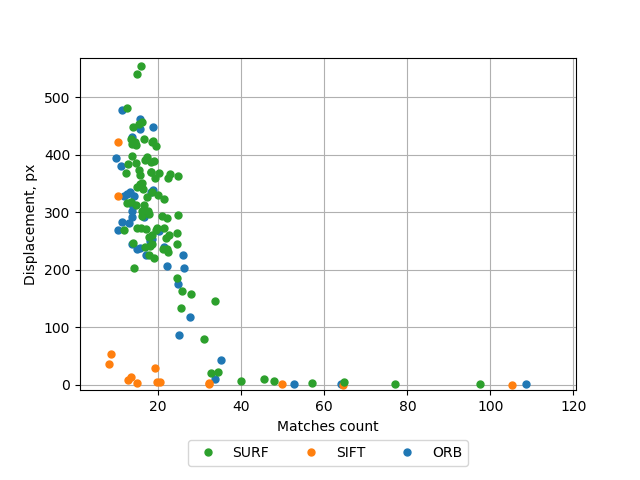
\includegraphics[width=0.6\textwidth,keepaspectratio]{ex2/sp/Rand_noises_d_by_m.png}      
		\centering\caption{  Изменение смещения с ростом числа точек при использовании шума соль-и-перец}
		\label{rand_noises_sp_b_by_m}                           
	\end{figure} 
	
	Зависимость смещения от количества найденных точек, как видно на графиках \ref{rand_noises_gauss_b_by_m}-\ref{rand_noises_sp_b_by_m}, выражена не так ярко, как при размытии, и можно наблюдать более плавный переход.
	
	Итак, наивысшая точность при применении случайных шумов достигается при использовании алгоритма SIFT. Наихудший результат показывает ORB. Стоит заметить, что и при использовании импульсного шума соль-перец, и при использовании аддитивного гауссовского шума наибольшие количества особых точек находит алгоритм SURF.
	
	Обобщая полученные результаты, можно сказать, что все рассмотренные алгоритмы проявили себя достаточно хорошо при тех уровнях зашумления, которые потенциально могут встретиться на практике. Значения, при которых наблюдается серьезное смещение относительно требуемого, в любом случае сделали бы на практике такую фотографию непригодной к использованию. 
	
	При размытии изображения наилучшим образом ведет себя алгоритм SURF, что позволяет рекомендовать его к использованию, если исходные фотографии сделаны с заметным нарушением фокусировки.
	При случайных шумах, как аддитивном, так и импульсном, наилучшим образом работает SIFT, ценой большего времени выполнения и вычислительной сложности. 
	Хуже всего в проведенных экспериментах отработал алгоритм ORB, в особенности, при использовании шума соль-перец.
}
\newpage


%------------------------------------------------
% Заключение
%------------------------------------------------

\titleformat{\section}{\large\bfseries\centering}{\thesection}{0.5em}{\MakeUppercase}
\titleformat{\subsection}[block]{\bfseries\hspace{1em}}{\thesubsection}{0.5em}{}

\newpage
\phantomsection
\addcontentsline{toc}{section}{Заключение}
\section*{Заключение}
{
    В ходе данной работы была рассмотрена задача сшивки изображения и методы ее решения. Проведен обзор математической постановки задачи. Рассмотрен алгоритм нахождения пространственного преобразования по опорным точкам. Был дан обзор нескольких методов поиска опорных точек, реализованных в открытой библиотеке OpenCV.
    
    Рассмотрены цифровые шумы в задачах обработки изображений и их особенности, разобраны популярные математические модели искусственно генерируемых шумов, используемых для тестирования алгоритмов и оборудования. 
    
    Реализована компьютерная программа, осуществляющая совмещение изображений по особым точкам с возможностью выбора типа дескриптора. Также, реализована программная среда для экспериментов, позволяющая использовать изображения с генерацией различных типов и уровней зашумления, формировать отчеты о работе алгоритмов и анализировать графическое представление результатов. 
    
    В ходе серии экспериментов было выяснено, что представленные алгоритмы являются достаточно устойчивыми к зашумлению, и работают с достаточной точностью при уровнях шума, допускающих сохранение практической ценности таких изображений. Однако, можно выделить алгоритмы, лучше или хуже ведущие себя при определенных типах шумов. Результаты экспериментов показывают, что наилучшим образом все представленные алгоритмы справились с размытием, наихудшим - с импульсным шумом. Были сделаны выводы о применимости отдельных алгоритмов при конкретных практически возможных дефектах фотографий. 
    
    Дальнейшим развитием работы видится оценка при использовании на зашумленных изображениях восстанавливающих фильтров, либо восстановления шума при помощи моделей глубокого обучения.
}

\newpage
\phantomsection
\addcontentsline{toc}{section}{Список использованных источников}
%------------------------------------------------
% Список литературы
%------------------------------------------------
\section*{Список использованных источников}
{
	\begin{enumerate}[label=\arabic*]
%	\item{Гонсалес Р., Вудс Р. Цифровая обработка изображений // М.: Техносфера. – 2005. – Т. 1072. – С. 2.}
	\item{Bres, S. Detection of interest points for image indexation [Текст] / S. Bres, J. M. Jolion // International Conference on Advances in Visual Information Systems. -- Springer, Berlin, Heidelberg, 1999. -- P. 427-435.}{\label{interest points}}	
	\item{Lowe, D. G. Distinctive image features from scale-invariant keypoints [Текст] / D. G. Lowe // International journal of computer vision. -- 2004. -- Vol. 60. -- I. 2. -- P. 91-110.}\label{lowe surf}
%	\item{Кудрина М. А., Мурзин А. В. Аффинные преобразования объектов в компьютерной графике // НиКа. 2014. №. URL: \\https://cyberleninka.ru/article/n/affinnye-preobrazovaniya-obektov-v-kompyuternoy-grafike (дата обращения: 25.12.2018). }
	\item{Rublee, E. ORB: an efficient alternative to SIFT or SURF [Текст] / E. Rublee, D. Brando, J. Joestar // ICCV '11 Proceedings of the 2011 International Conference on Computer Vision. -- IEEE Computer Society Washington, DC, USA, 2011. -- P. 2564-2571. }\label{rublee orb}
	\item{Проективное преобразование [Электронный ресурс] // Википедия : свободная энцикл. -- Электрон. дан. -- 2019. -- URL: \\https://ru.wikipedia.org/?oldid=99107559 (дата обращения: 15.04.2019).}\label{wiki projective}
	\item{Аффинное преобразование [Электронный ресурс] // Википедия : свободная энцикл. -- Электрон. дан. -- 2019. -- URL: \\https://ru.wikipedia.org/?oldid=93707864 (дата обращения: 15.04.2019).}\label{wiki affine}
	\item {Karami, E. Image Matching Using SIFT, SURF, BRIEF and ORB: Per-\\formance Comparison for Distorted Images [Электронный ресурс] / E. Karami, S. Prasad, M. Shehata // arXiv preprint. -- 2015. -- Электрон. дан. -- URL:\\ https://arxiv.org/ftp/arxiv/papers/1710/1710.02726.pdf\quad (дата обращения:\\ 25.05.2019).}
	\item{Kong, H. A generalized Laplacian of Gaussian filter for blob detection and its applications [Текст] / H. Kong, H. C. Akakin, S. E. Sarma // IEEE transactions on cybernetics. -- IEEE Computer Society Washington, DC, USA, 2013. -- V. 43. -- I. 6. -- P. 1719-1733.}{\label{imagematching paper}}
%	\item{Бинарное изображение // Википедия. [2018—2018]. Дата обновления: 30.05.2018. URL: https://ru.wikipedia.org/?oldid=92976723 \\(дата обращения: 30.05.2018).}
	\item{Moeslund, T. B. BLOB Analysis: An introduction to video and image processing [Текст] / T. B. Moeslund. -- Springer, London, 2012. -- 227 p. -- p. 5-20.}{\label{blobs}}
	\item{Цифровой шум изображения  [Электронный ресурс] // Википедия : свободная энцикл. -- Электрон. дан. -- 2019. -- URL:\\ https://ru.wikipedia.org/?oldid=95235149 (дата обращения: 15.04.2019).}\label{wiki noise}
	\item{Deng, G. An adaptive Gaussian filter for noise reduction and edge detection [Текст] / G. Deng, L. W. Cahill // IEEE Conference Record. -- IEEE Computer Society Washington, DC, USA, 1993. -- P. 1615-1619.}{\label{gaussian filter}}
b 	\item{OpenCV Documentation [Электронный ресурс] : официальная документация библиотеки OpenCV. / Intel Corporation, Willow Garage Inc., Itseez Ltd. -- Электрон. дан. -- 2019. -- URL: \\https://docs.opencv.org (дата обращения: 25.04.2019). }{\label{cv docs}}
\end{enumerate}


%--------------------------------
% Приложения. Коды программ и.т.д.
%--------------------------------
\newpage
\phantomsection
\addcontentsline{toc}{section}{Приложение А Код программы}

\section*{Приложение А}
{
	\begin{center}
	\textbf{Код программы}
	\end{center}
%	Файл stitching.py:
	\lstinputlisting[language=python,mathescape=true]{./src/stitching.py}
	\newpage
	%\lstinputlisting[language=python,mathescape=true]{./src/test.py}
}

\end{document}
